\documentclass{beamer}
%
% Choose how your presentation looks.
%
% For more themes, color themes and font themes, see:
% http://deic.uab.es/~iblanes/beamer_gallery/index_by_theme.html
%
\mode<presentation>
{
  \usetheme{Boadilla}      % or try Darmstadt, Madrid, Warsaw, ...
  \usecolortheme{beaver} % or try albatross, beaver, crane, ...
  \usefonttheme{default}  % or try serif, structurebold, ...
  \useoutertheme{split}
  \setbeamertemplate{navigation symbols}{}
  \setbeamertemplate{caption}[numbered]
}

\usepackage[english]{babel}
\usepackage[utf8x]{inputenc}

\usepackage[justification=centering,font=scriptsize]{caption}

\captionsetup{labelformat=empty}

\usepackage{amsmath}
\usepackage{tikz}
\usepackage{mathtools}

\newcommand{\tikzmark}[2]{
    \tikz[overlay,remember picture,baseline]
    \node[anchor=base] (#1){$#2$};
}

\title[Implementation and Visualization of the ChaCha Cipher Family in CrypTool 2]{Implementation and Didactical Visualization of the ChaCha Cipher Family in CrypTool 2}
\author{Ramdip Gill}
\institute{Universität Heidelberg}
\date{28. Januar 2021}

\setbeamertemplate{headline}{}
\setbeamertemplate{footline}
{
  \leavevmode%
  \hbox{%
  \begin{beamercolorbox}[wd=.2\paperwidth,ht=2.25ex,dp=1ex,center]{author in head/foot}%
    \usebeamerfont{author in head/foot}\insertauthor
  \end{beamercolorbox}%
  \begin{beamercolorbox}[wd=.6\paperwidth,ht=2.25ex,dp=1ex,center]{title in head/foot}%
    \usebeamerfont{title in head/foot}\insertshorttitle
  \end{beamercolorbox}%
  \begin{beamercolorbox}[wd=.2\paperwidth,ht=2.25ex,dp=1ex,right]{author in head/foot}%
    \usebeamerfont{date in head/foot} \insertframenumber{} / \inserttotalframenumber\hspace*{2ex}
  \end{beamercolorbox}
  }%
  \vskip0pt%
}

\urlstyle{same}

\begin{document}

\begin{frame}[plain]
  \titlepage
\end{frame}

% Uncomment these lines for an automatically generated outline.
\begin{frame}[plain]{Outline}
  \tableofcontents
\end{frame}

\section{Einleitung}

\subsection{CrypTool 2}
\begin{frame}{CrypTool 2}
\begin{figure}
\center
\begin{minipage}{.6\textwidth}
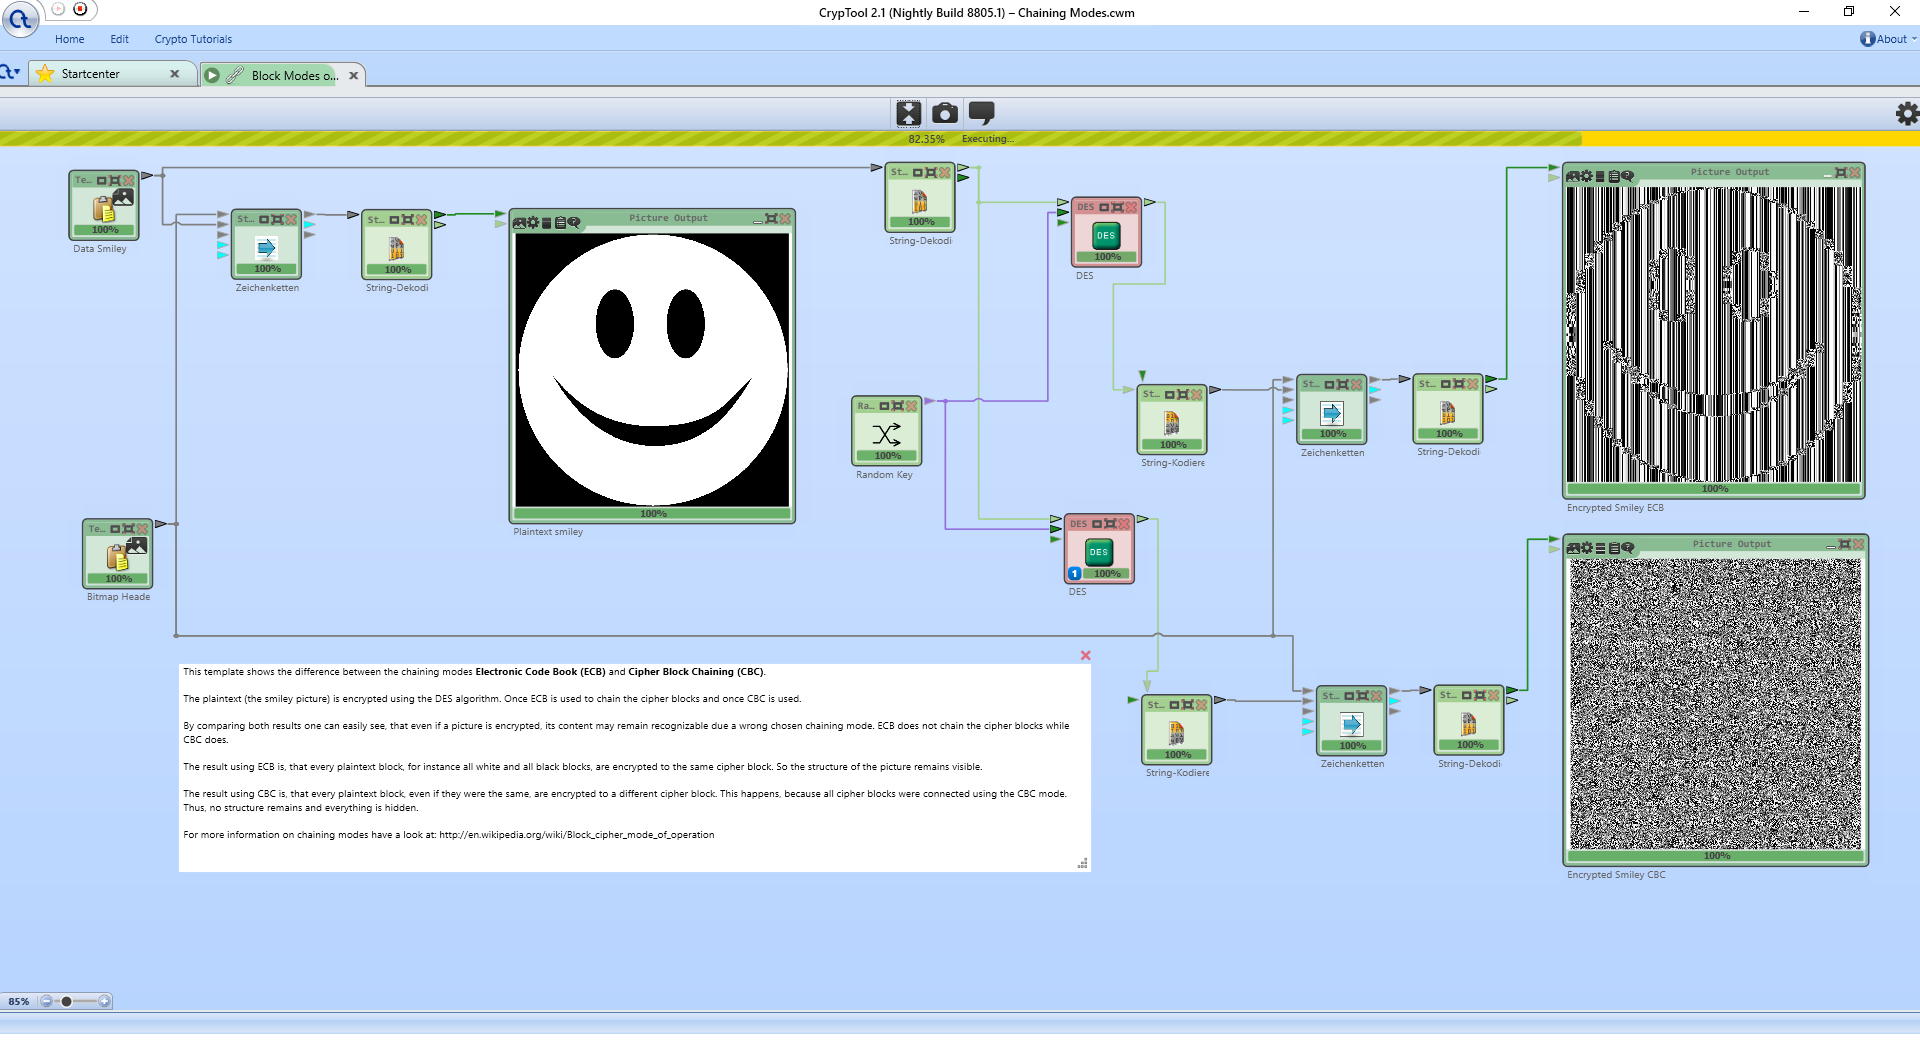
\includegraphics[width=\textwidth]{figures/010_Block_Modes_Symmetric_Ciphers.png}
\end{minipage}
\caption{CrypTool 2\\(Demonstration Electronic Code Book (ECB) vs. Cipher Block Chaining (CBC) Modus)}
\end{figure}
\begin{itemize}
\item kostenlose Open-Source E-Learning-Plattform\\für Kryptographie und Kryptoanalyse
\item benutzt Konzepte der visuellen Programmierung
\item beinhaltet unter anderem schon Visualisierungen \\von Chiffren wie AES, DES etc.
\item Projektleiter von CT2 ist von der Universität Siegen
\end{itemize}
\end{frame}

\subsection{ChaCha}
\begin{frame}{ChaCha}
\renewcommand*{\thefootnote}{\fnsymbol{footnote}}
\begin{figure}
\center
\begin{minipage}{.25\textwidth}
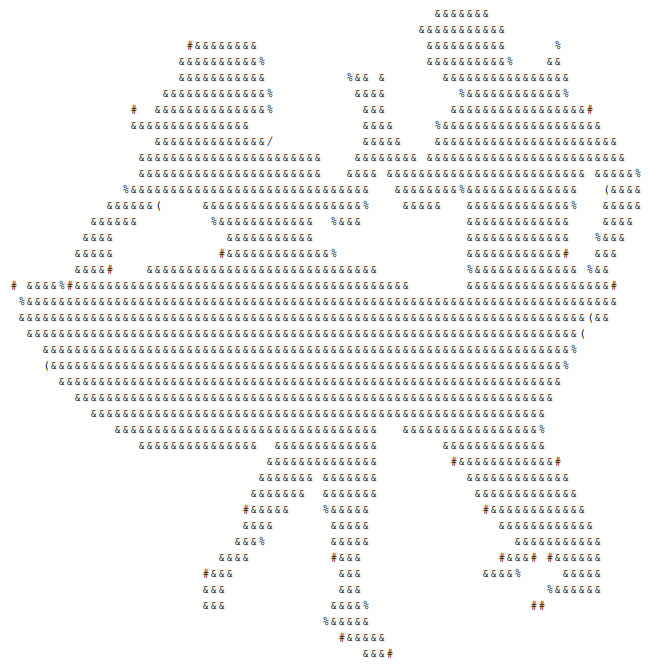
\includegraphics[width=\textwidth]{figures/chacha-ascii-art/chacha-ascii-art.png}
\end{minipage}
\end{figure}
\begin{itemize}
\item 256-bit Stromchiffre
\item veröffentlicht in 2008 von Daniel J. Bernstein
\item basiert auf Salsa20 des gleichen Autors
\item wird seit 2014 im Transport Layer Security Protokoll (TLS) \\eingesetzt aufgrund besserer Geschwindigkeit\footnotemark\  gegenüber AES-GCM
\item immun gegen bisherige TLS-Angriffe \\(Timing-Attack, Padding-Oracle-Attack)\\ $\Rightarrow$\ sehr relevant für moderne Kryptographie
\end{itemize}
\footnotetext[1]{in Software-Implementierungen}
\end{frame}

\section{Ziele des Plugins}
\begin{frame}{Ziele des Plugins}
\begin{itemize}
\item Unterstützung für 128-bit und 256-bit Schlüssel
\item Unterstützung für alle Chiffren der Familie (8, 12, 20 Runden)
\item Unterstützung für beide existierende Versionen: \\64-bit Zähler mit 64-bit Initialisierungsvektor (originale Version) und 32-bit Zähler mit 96-bit Initialisierungsvektor \\(Version der Internet Engineering Task Force)
\item Visualisierung des Ver-/Entschlüsselungsprozesses
\item Visualisierung der Diffusion
\item Fokus auf Didaktik
\end{itemize}
\end{frame}

\section{ChaCha-Spezifikation}
\begin{frame}{ChaCha-Spezifikation}

\begin{center}
\parbox{0.8\textwidth}{
\textbf{Abstract.} ChaCha8 is a 256-bit stream cipher based on the 8-round
cipher Salsa20/8. The changes from Salsa20/8 to ChaCha8 are designed
to improve diffusion per round, conjecturally increasing resistance to
cryptanalysis, while preserving—and often improving—time per round. [...]
\vspace{-0.75em}
\begin{flushright}
-- Daniel J. Bernstein
\end{flushright}
}
\end{center}
\begin{itemize}
\item Quelle: \url{https://cr.yp.to/chacha/chacha-20080120.pdf}
\item erläutert lediglich Unterschiede zu Salsa20
\item Unterschiede: Zustandsmatrix-Aufbau und Quarterround-Funktion
\end{itemize}
\end{frame}

\subsection{Aufbau der Zustandsmatrix}
\begin{frame}{Aufbau der Zustandsmatrix (ChaCha)}
\begin{equation*}
\begin{pmatrix}
\texttt{CONSTANT}& \texttt{CONSTANT} & \texttt{CONSTANT} & \texttt{CONSTANT} \\
\texttt{KEY} & \texttt{KEY} & \texttt{KEY} & \texttt{KEY} \\
\texttt{KEY} & \texttt{KEY} & \texttt{KEY} & \texttt{KEY} \\
\texttt{COUNTER} & \texttt{COUNTER} & \texttt{IV} & \texttt{IV} \\
\end{pmatrix}
\end{equation*}
\begin{itemize}
\item 32-bit pro Eintrag (insgesamt: 512-bit)
\item Konstanten abhängig von Schlüssellänge
\begin{itemize}
\item 128-bit Schlüssel: ``expand 16-byte k'' (ASCII) \\
$\Rightarrow$ \texttt{65:78:70:61 6e:64:20:31 36:2d:62:79 74:65:20:6b} (hex)
\item 256-bit Schlüssel: ``expand 32-byte k'' (ASCII) \\
$\Rightarrow$ \texttt{65:78:70:61 6e:64:20:33 32:2d:62:79 74:65:20:6b} (hex)
\end{itemize}
\item 128-bit Schlüssel werden konkateniert mit sich selbst
\item Byte-Reihenfolge aller 32-bit Blöcke wird umgekehrt
\item Zähler: Byte-Reihenfolge wird zusätzlich erst komplett umgedreht
\end{itemize}
\end{frame}

\begin{frame}{Aufbau der Zustandsmatrix -- Beispiel}
Schlüssel (256-bit): \\
\hspace{1em} \texttt{00:01:02:03 04:05:06:07 08:09:0a:0b 0c:0d:0e:0f} \\
\hspace{1em} \texttt{10:11:12:13 14:15:16:17 18:19:1a:1b 1c:1d:1e:1f} \\
$\Rightarrow$ Konstanten (128-bit): \\
\hspace{1em} \texttt{65:78:70:61 6e:64:20:33 32:2d:62:79 74:65:20:6b} \\
Initialisierungsvektor (64-bit): \\
\hspace{1em} \texttt{00:11:22:33 44:55:66:77} \\
Zähler (64-bit): \\
\hspace{1em} \texttt{00:00:00:00 00:00:00:01} \\
\vspace{1em} $\Rightarrow$ Zustandsmatrix:
\begin{equation*}
\begin{pmatrix}
\texttt{61:70:78:65}& \texttt{33:20:64:6e} & \texttt{79:62:2d:32} & \texttt{6b:20:65:74} \\
\texttt{03:02:01:00} & \texttt{07:06:05:04} & \texttt{0b:0a:09:08} & \texttt{0f:0e:0d:0c} \\
\texttt{13:12:11:10} & \texttt{17:16:15:14} & \texttt{1b:1a:19:18} & \texttt{1f:1e:1d:1c} \\
\texttt{00:00:00:01} & \texttt{00:00:00:00} & \texttt{33:22:11:00} & \texttt{77:66:55:44} \\
\end{pmatrix}
\end{equation*}
\end{frame}

\begin{frame}{Aufbau der Zustandsmatrix -- Plugin}
\begin{figure}
\center
\begin{minipage}{\textwidth}
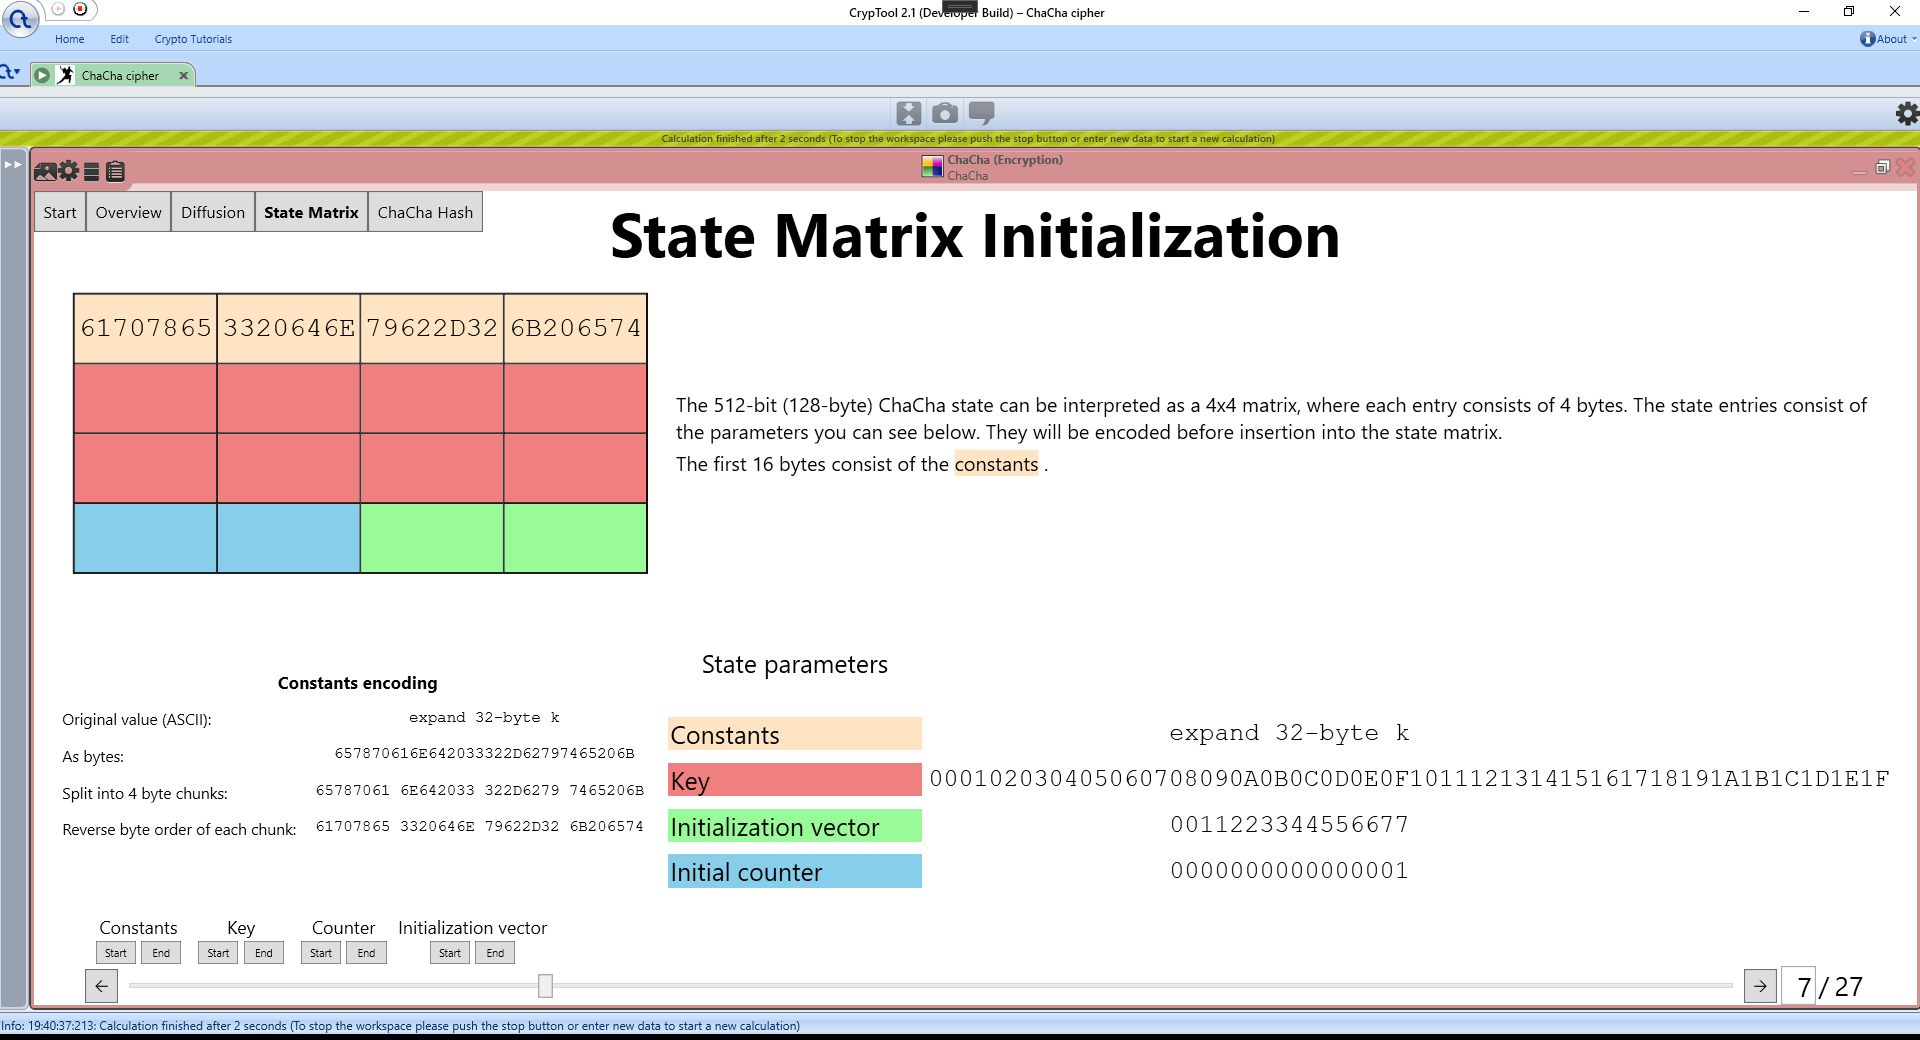
\includegraphics[width=\textwidth]{figures/state-matrix/1-state-matrix-constants.png}
\end{minipage}
\end{figure}
\end{frame}

\begin{frame}{Aufbau der Zustandsmatrix -- Plugin}
\begin{figure}
\center
\begin{minipage}{\textwidth}
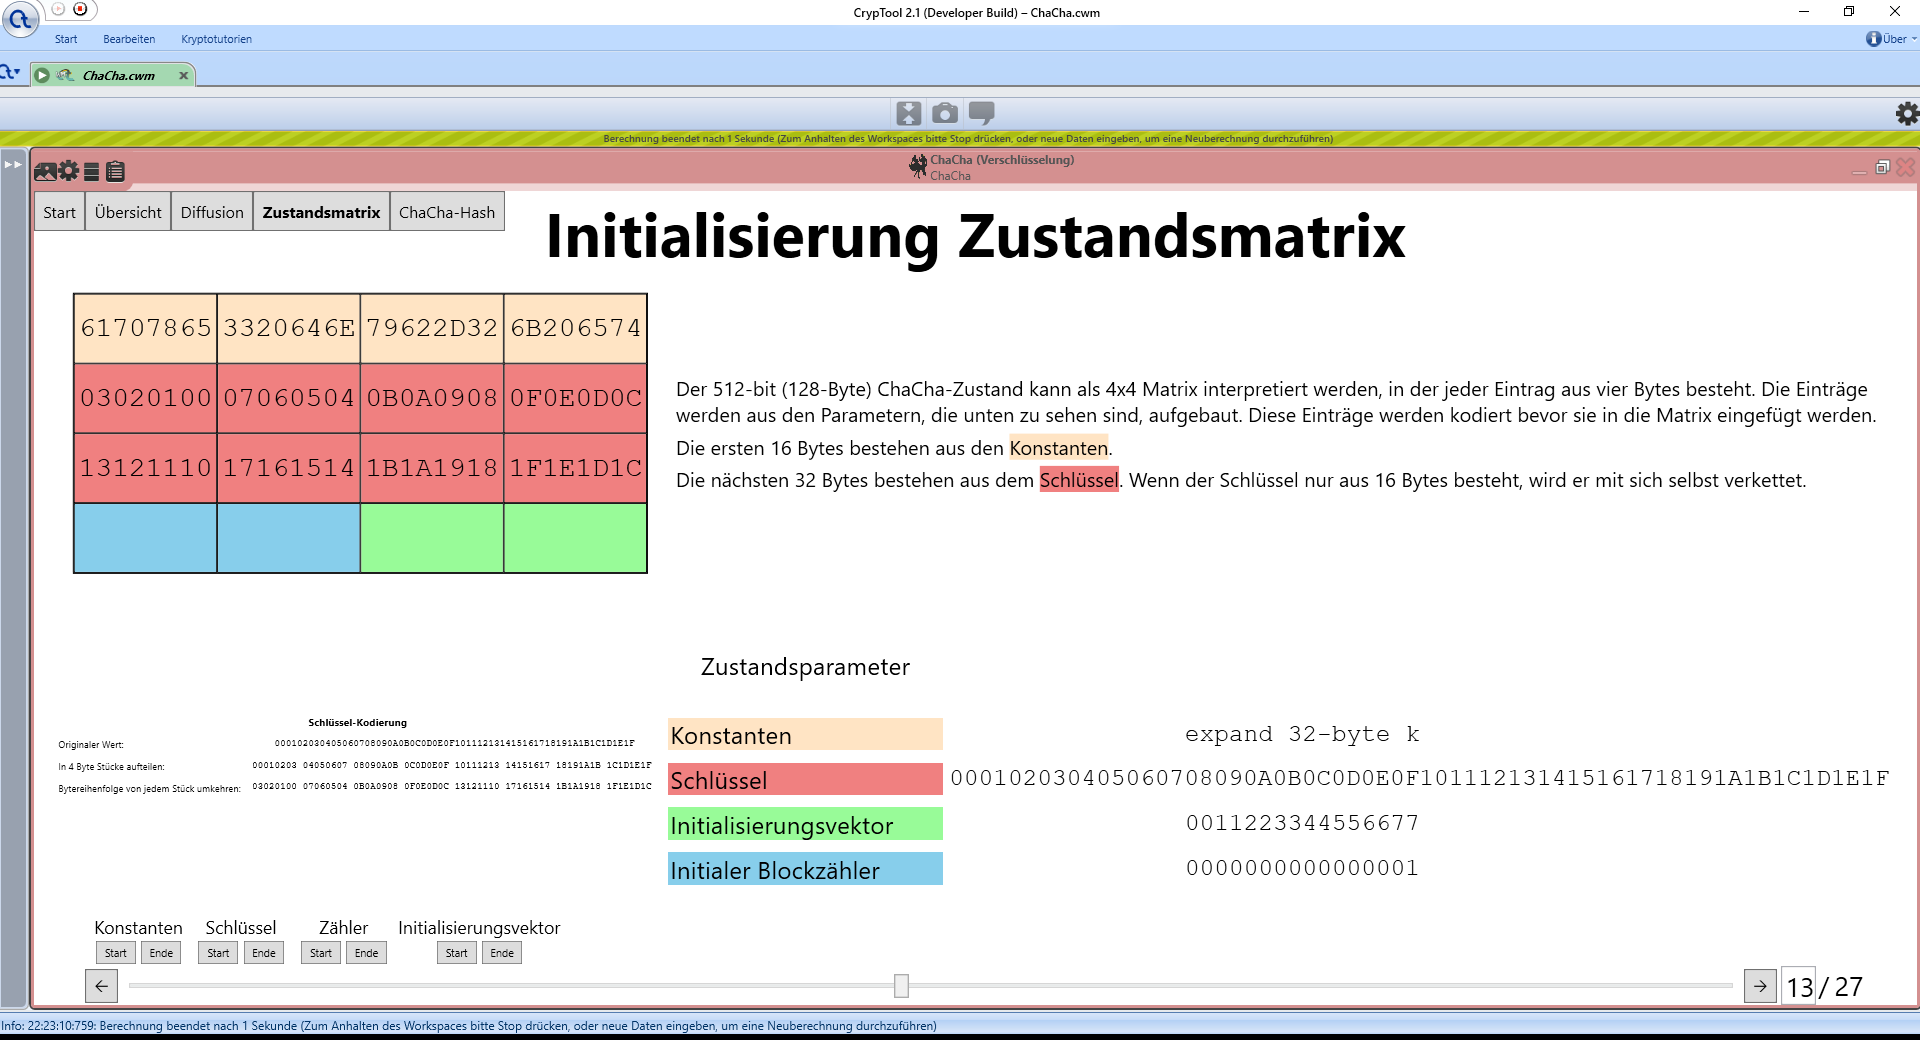
\includegraphics[width=\textwidth]{figures/state-matrix/2-state-matrix-key.png}
\end{minipage}
\end{figure}
\end{frame}

\begin{frame}{Aufbau der Zustandsmatrix -- Plugin}
\begin{figure}
\center
\begin{minipage}{\textwidth}
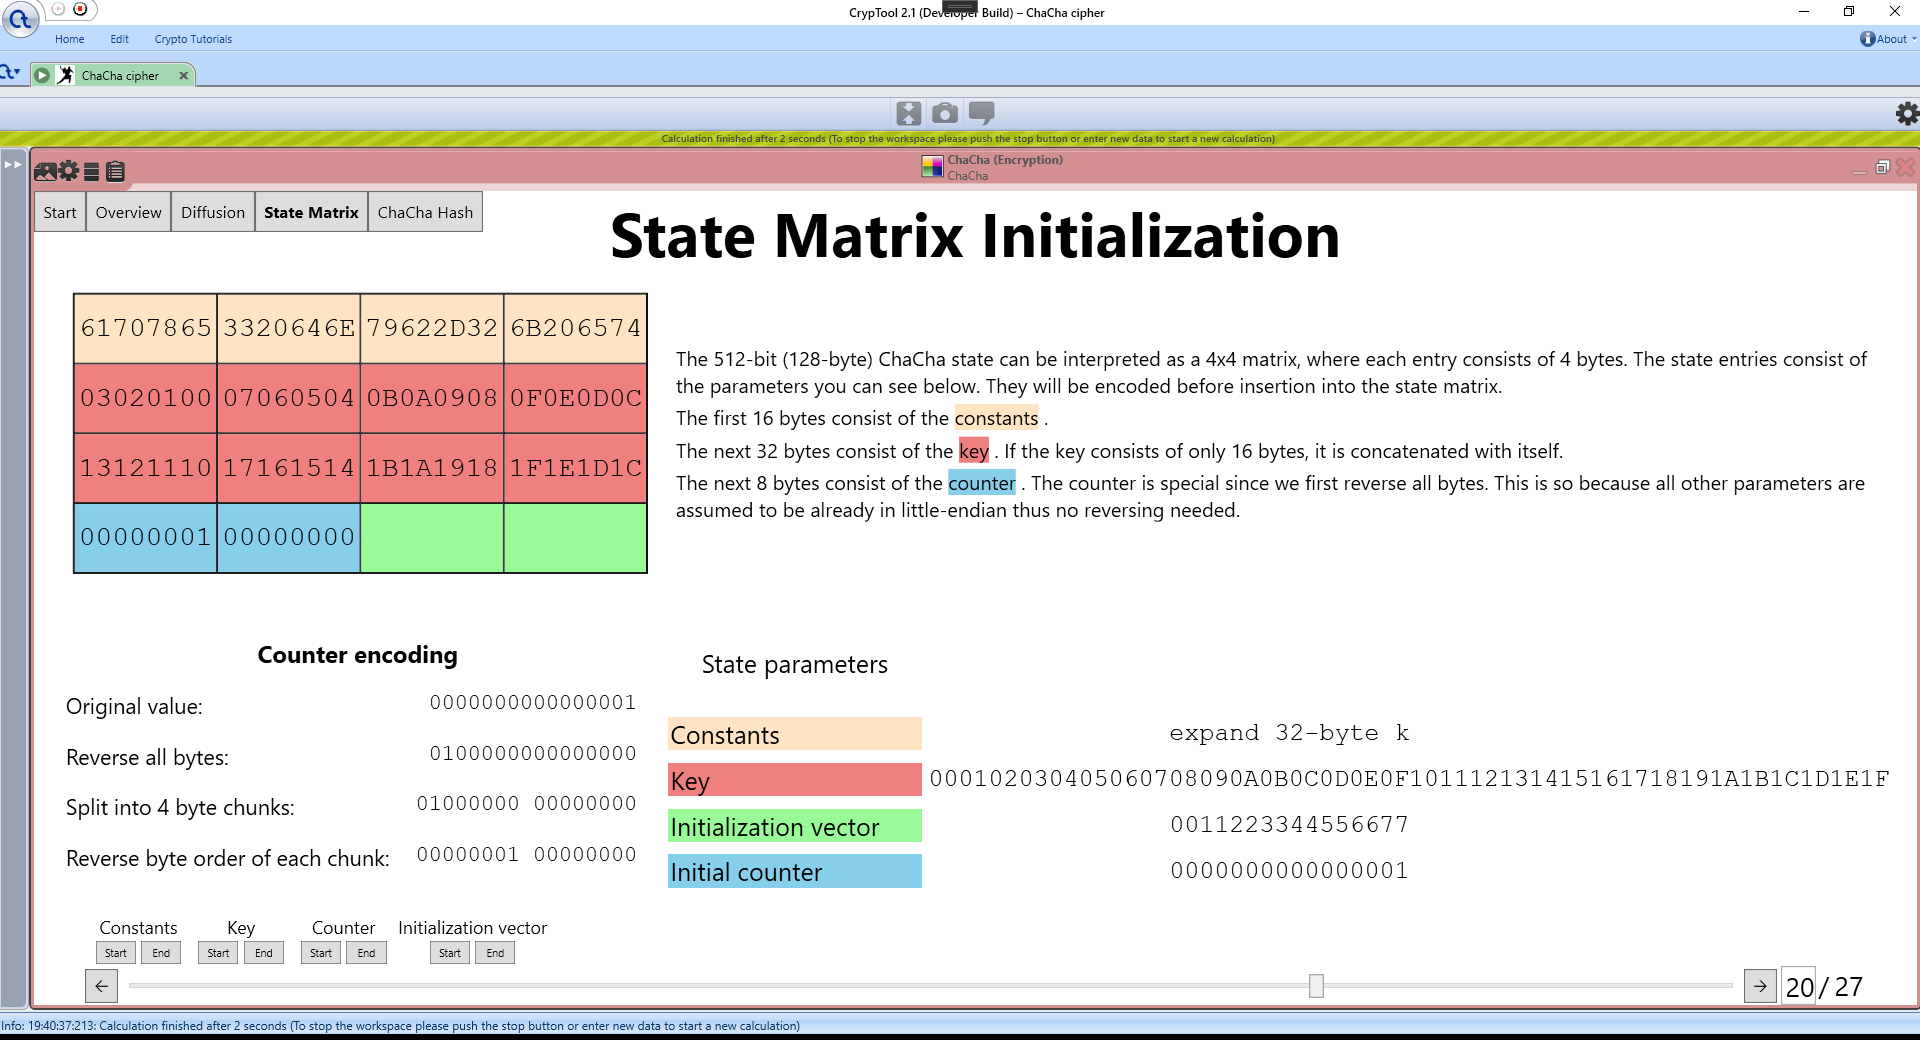
\includegraphics[width=\textwidth]{figures/state-matrix/3-state-matrix-counter.png}
\end{minipage}
\end{figure}
\end{frame}

\begin{frame}{Aufbau der Zustandsmatrix -- Plugin}
\begin{figure}
\center
\begin{minipage}{\textwidth}
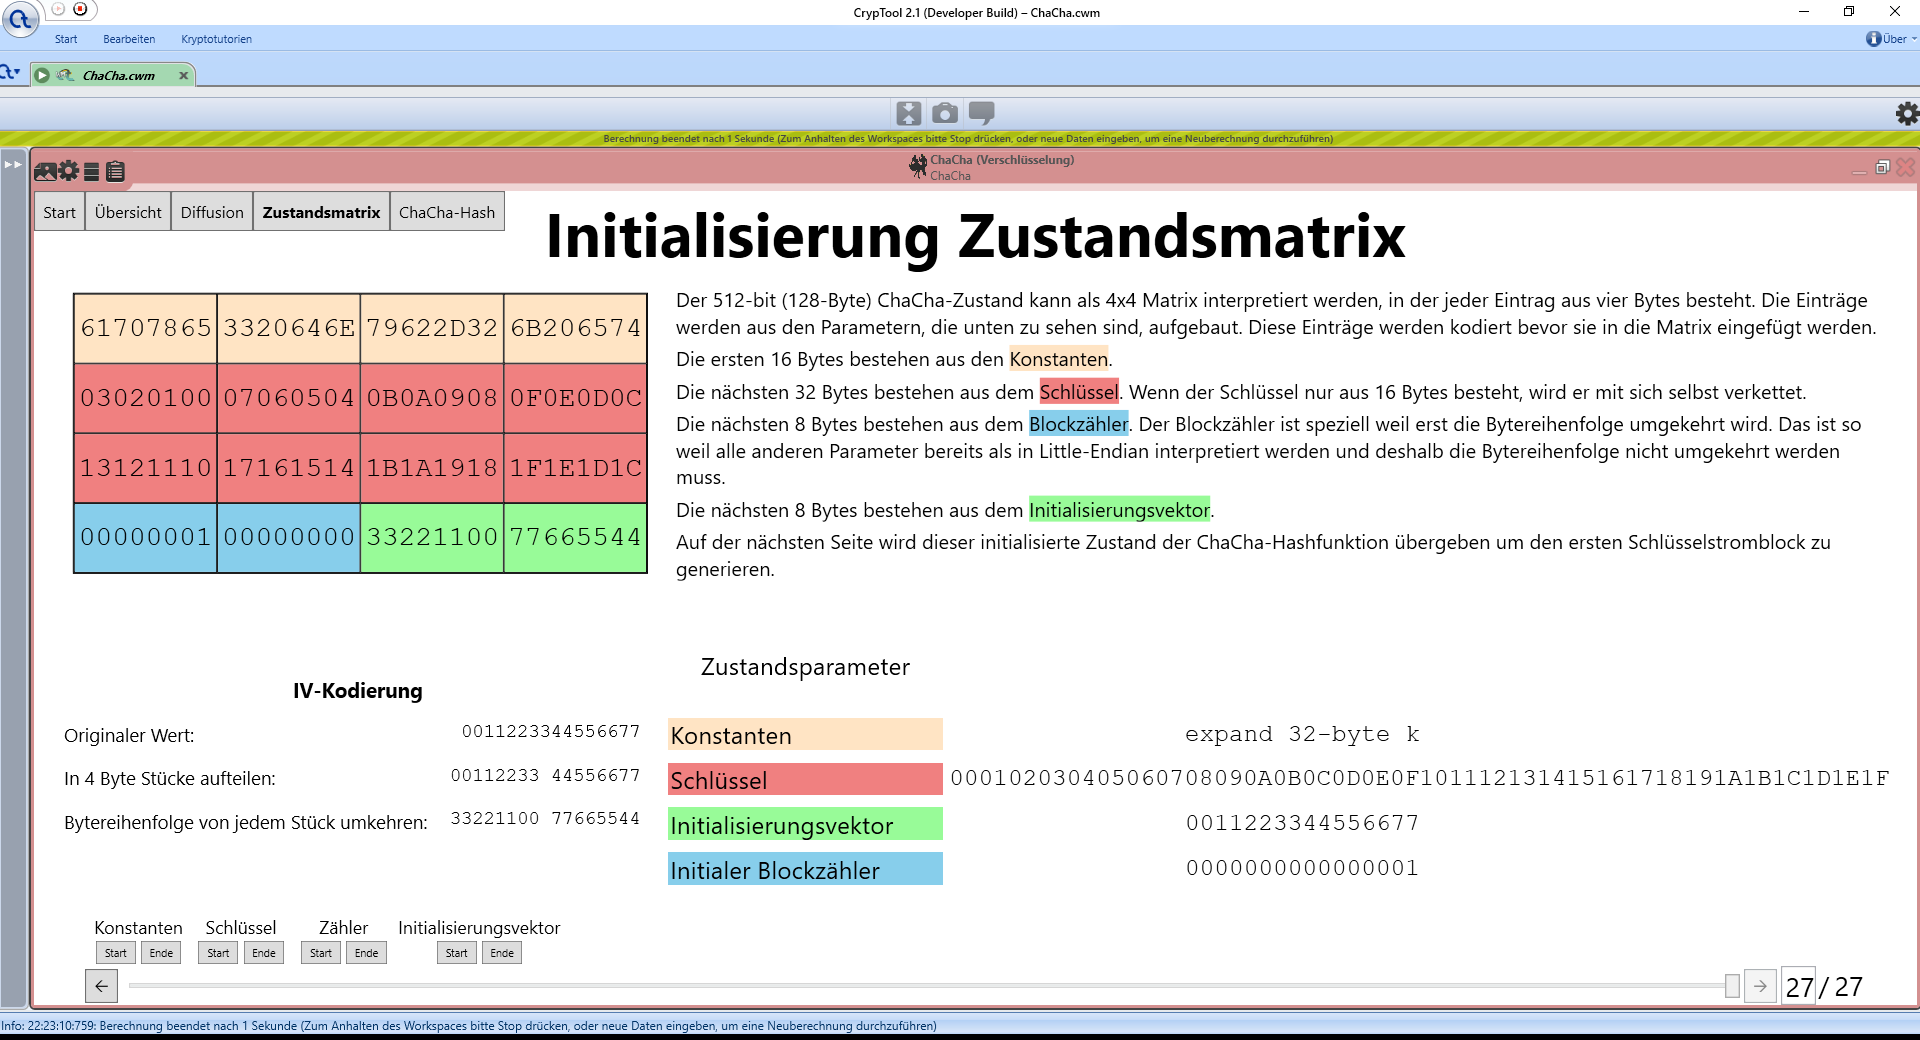
\includegraphics[width=\textwidth]{figures/state-matrix/4-state-matrix-iv.png}
\end{minipage}
\end{figure}
\end{frame}

\subsection{Quarterround-Funktion}
\begin{frame}[fragile]{Quarterround-Funktion}
\begin{center}
\begin{minipage}{0.5\linewidth}
\texttt{quarterround(a,b,c,d):} \\
\hspace*{2em}\texttt{a += b; d  \^{}= a; d} \verb|<<<|\texttt{= 16} \\
\hspace*{2em}\texttt{c += d; b \^{}= c; b} \verb|<<<|\texttt{= 12} \\
\hspace*{2em}\texttt{a += b; d \^{}= a; d} \verb|<<<|\texttt{= 8} \\
\hspace*{2em}\texttt{c += d; b \^{}= c; b} \verb|<<<|\texttt{= 7} \\
\hspace*{2em}\texttt{return a, b, c, d}
\end{minipage}
\end{center}
\begin{itemize}
\item modifiziert vier 32-bit Matrixeinträge
\item pro Runde: vier Aufrufe der Quarterround-Funktion \\
$\Rightarrow$ nach jeder Runde wurden alle Matrixeinträge modifiziert
\item Runden werden aufgeteilt in \textit{Spalten-} und \textit{Diagonalrunden}
\end{itemize}
\end{frame}

\begin{frame}{Quarterround-Funktion -- Spaltenrunde}
\begin{equation*}
\begin{pmatrix}
\hspace{0.2em}\tikzmark{0}{y_0} & y_1 & y_2 & y_3 \\
\hspace{0.2em}y_4 &y_5 & y_6 & y_7 \\
\hspace{0.2em}y_8 & y_9 & y_{10} & y_{11} \\
\hspace{0.2em}\tikzmark{12}{y_{12}} & y_{13} & y_{14} & y_{15} \\
\end{pmatrix}
\begin{tikzpicture}[overlay,remember picture]
     \draw[opacity=.2,line width=3mm,line cap=round,color=green] (0.center) -- (12.center);
\end{tikzpicture}
\begin{pmatrix}
y_0 & \tikzmark{1}{y_1} & y_2 & y_3 \\
y_4 &y_5 & y_6 & y_7 \\
y_8 & y_9 & y_{10} & y_{11} \\
y_{12} & \tikzmark{13}{y_{13}} & y_{14} & y_{15} \\
\end{pmatrix}
\begin{tikzpicture}[overlay,remember picture]
     \draw[opacity=.2,line width=3mm,line cap=round,color=green] (1.center) -- (13.center);
\end{tikzpicture}
\end{equation*}
\begin{equation*}
\begin{pmatrix}
y_0 & y_1 & \tikzmark{2}{y_2} & y_3 \\
y_4 &y_5 & y_6 & y_7 \\
y_8 & y_9 & y_{10} & y_{11} \\
y_{12} & y_{13} & \tikzmark{14}{y_{14}} & y_{15} \\
\end{pmatrix}
\begin{tikzpicture}[overlay,remember picture]
     \draw[opacity=.2,line width=3mm,line cap=round,color=green] (2.center) -- (14.center);
\end{tikzpicture}
\begin{pmatrix}
y_0 & y_1 & y_2 & \tikzmark{3}{y_3} \\
y_4 &y_5 & y_6 & y_7 \\
y_8 & y_9 & y_{10} & y_{11} \\
y_{12} & y_{13} & y_{14} & \tikzmark{15}{y_{15}} \\
\end{pmatrix}
\end{equation*}
\begin{tikzpicture}[overlay,remember picture]
     \draw[opacity=.2,line width=3mm,line cap=round,color=green] (3.center) -- (15.center);
\end{tikzpicture}
\end{frame}

\begin{frame}{Quarterround-Funktion -- Diagonalrunde}
\begin{equation*}
\begin{pmatrix}
\tikzmark{0}{y_0} & y_1 & y_2 & y_3 \\
y_4 &y_5 & y_6 & y_7 \\
y_8 & y_9 & y_{10} & y_{11} \\
y_{12} & y_{13} & y_{14} & \tikzmark{15}{y_{15}} \\
\end{pmatrix}
\begin{tikzpicture}[overlay,remember picture]
     \draw[opacity=.2,line width=3mm,line cap=round,color=green] (0.center) -- (15.center);
\end{tikzpicture}
\begin{pmatrix}
\hspace{0.2em}y_0 & \tikzmark{1}{y_1} & y_2 & y_3 \\
\hspace{0.2em}y_4 &y_5 & y_6 & y_7 \\
\hspace{0.2em}y_8 & y_9 & y_{10} & \tikzmark{11}{y_{11}} \\
\hspace{0.2em}\tikzmark{12}{y_{12}} & y_{13} & y_{14} & y_{15} \\
\end{pmatrix}
\begin{tikzpicture}[overlay,remember picture]
     \draw[opacity=.2,line width=3mm,line cap=round,color=green] (1.center) -- (11.center);
     \draw[opacity=.2,line width=3mm,line cap=round,color=green] (12.center) -- (12.center);
\end{tikzpicture}
\end{equation*}
\begin{equation*}
\begin{pmatrix}
y_0 & y_1 & \tikzmark{2}{y_2} & y_3 \\
y_4 &y_5 & y_6 & \tikzmark{7}{y_7} \\
\tikzmark{8}{y_8} & y_9 & y_{10} & y_{11} \\
y_{12} & \tikzmark{13}{y_{13}} & y_{14} & y_{15} \\
\end{pmatrix}
\begin{tikzpicture}[overlay,remember picture]
     \draw[opacity=.2,line width=3mm,line cap=round,color=green] (2.center) -- (7.center);
     \draw[opacity=.2,line width=3mm,line cap=round,color=green] (8.center) -- (13.center);
\end{tikzpicture}
\begin{pmatrix}
y_0 & y_1 & y_2 & \tikzmark{3}{y_3} \\
\tikzmark{4}{y_4} &y_5 & y_6 & y_7 \\
y_8 & \tikzmark{9}{y_9} & y_{10} & y_{11} \\
y_{12} & y_{13} & \tikzmark{14}{y_{14}} & y_{15} \\
\end{pmatrix}
\end{equation*}
\begin{tikzpicture}[overlay,remember picture]
     \draw[opacity=.2,line width=3mm,line cap=round,color=green] (3.center) -- (3.center);
     \draw[opacity=.2,line width=3mm,line cap=round,color=green] (4.center) -- (14.center);
\end{tikzpicture}
\end{frame}

\subsection{Hashfunktion}
\begin{frame}{Hashfunktion}
\begin{center}
\begin{minipage}{\linewidth}
\scriptsize
\texttt{chachahash(y):} \\
\hspace*{2em}\texttt{z = copy(y)}\\
\hspace*{2em}\texttt{for(i = 0; i < ROUNDS; i += 2) \{}\\
\hspace*{4em}\texttt{// column round}\\
\hspace*{4em}\texttt{y[0], y[4], y[8], \ y[12] = quarterround(y[0], y[4], y[8], \  y[12])}\\
\hspace*{4em}\texttt{y[1], y[5], y[9], \ y[13] = quarterround(y[1], y[5], y[9], \  y[13])}\\
\hspace*{4em}\texttt{y[2], y[6], y[10], y[14] = quarterround(y[2], y[6], y[10], y[14])}\\
\hspace*{4em}\texttt{y[3], y[7], y[11], y[15] = quarterround(y[3], y[7], y[11], y[15])}\\
\hspace*{4em}\texttt{// diagonal round}\\
\hspace*{4em}\texttt{y[0], y[5], y[10], y[15] = quarterround(y[0], y[5], y[10], y[15])}\\
\hspace*{4em}\texttt{y[1], y[6], y[11], y[12] = quarterround(y[0], y[5], y[10], y[15])}\\
\hspace*{4em}\texttt{y[2], y[7], y[8], \  y[13] = quarterround(y[0], y[5], y[10], y[15])}\\
\hspace*{4em}\texttt{y[3], y[4], y[9], \  y[14] = quarterround(y[0], y[5], y[10], y[15])}\\
\hspace*{2em}\texttt{\}}\\
\hspace*{2em}\texttt{for(i = 0; i < 16; i += 1) \{}\\
\hspace*{4em}\texttt{y[i] += z[i]}\\
\hspace*{4em}\texttt{y[i] = littleendian(y[i])}  // reverse byte order\\
\hspace*{2em}\texttt{\}}\\
\hspace*{2em}\texttt{return y}
\end{minipage}
\end{center}
\end{frame}

\begin{frame}{Hashfunktion -- Plugin}
\begin{figure}
\center
\begin{minipage}{\textwidth}
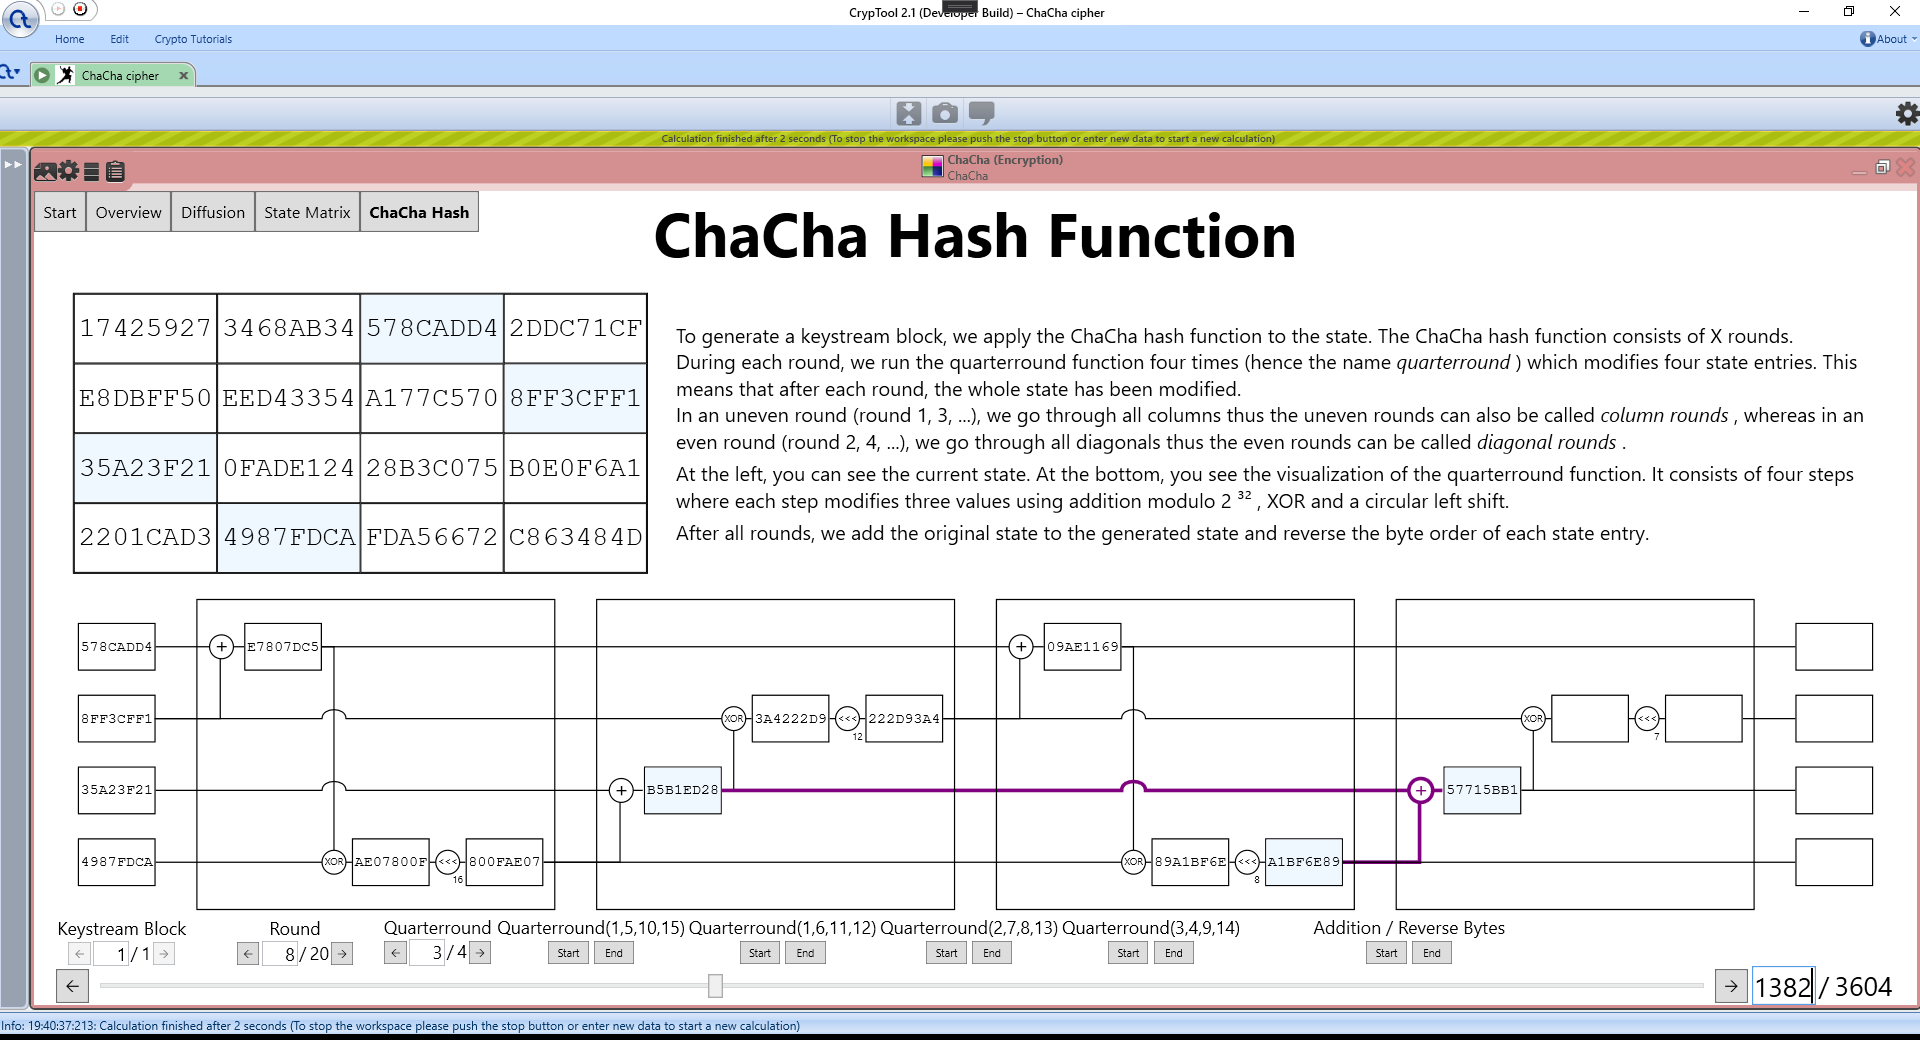
\includegraphics[width=\textwidth]{figures/chachahash/chachahash-mid-qr.png}
\end{minipage}
\end{figure}
\end{frame}

\begin{frame}{Hashfunktion -- Plugin}
\begin{figure}
\center
\begin{minipage}{\textwidth}
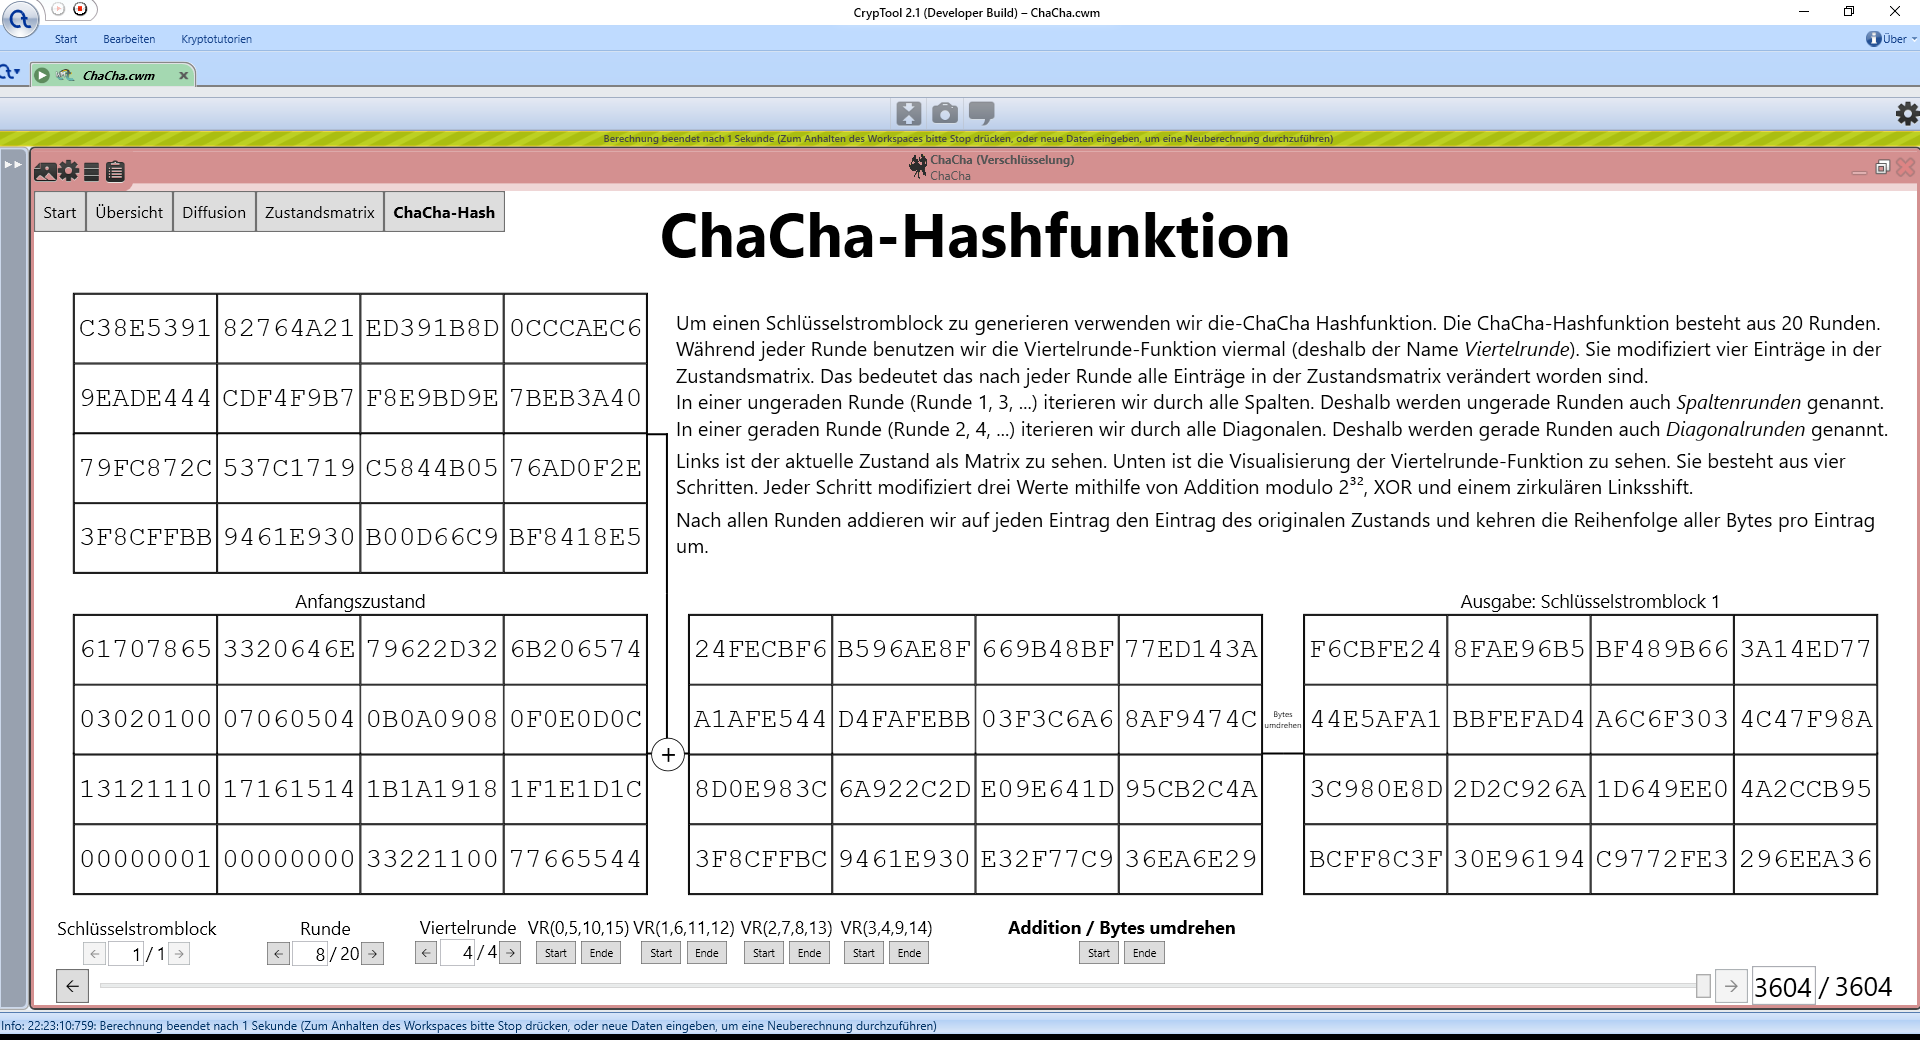
\includegraphics[width=\textwidth]{figures/chachahash/chachahash-end.png}
\end{minipage}
\end{figure}
\end{frame}

\section{Live-Präsentation des Plugins}
\begin{frame}{Live-Präsentation des Plugins}
\begin{figure}
\center
\begin{minipage}{.45\textwidth}
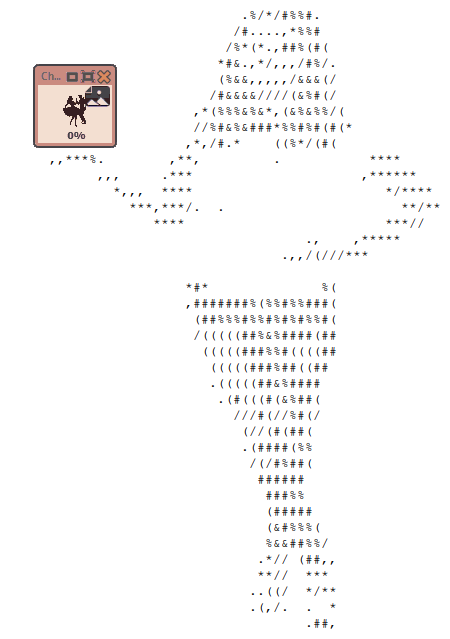
\includegraphics[width=\textwidth]{figures/presenting-plugin/presenting-plugin-composition.png}
\end{minipage}
\end{figure}
\end{frame}

\section{Zusammenfassung}
\begin{frame}{Zusammenfassung}
Ziele wurden wie folgt erreicht:
\begin{itemize}
\item Unterstützung für unterschiedliche Rundenanzahl sowie DJB- und IETF-Version
\begin{itemize}
\item entsprechende Optionen in den Plugin-Einstellungen
\item Inputvalidierung
\end{itemize}
\item Unterstützung für unterschiedliche Schlüsselgrößen \\
\begin{itemize}
\item Inputvalidierung (128-bit und 256-bit Schlüssel sind valide)
\item entsprechende Handhabung der Schlüsselgrößen entsprechend der Spezifikation
\end{itemize}
\item Visualisierung des Ver-/Entschlüsselungsprozesses \\
\begin{itemize}
\item Visualisierung des Aufbaus der Zustandsmatrix
\item Visualisierung der ChaCha-Hashfunktion
\end{itemize}
\item Visualisierung der Diffusion
\begin{itemize}
\item Dedizierte Seite für DIffusionseinstellungen
\item Zweitwerte werden untereinander angezeigt (Unterschiede rot markiert)
\item Anzahl der geflippten Bits wird absolut und in Prozent angezeigt
\end{itemize}
\end{itemize}
\end{frame}

\begin{frame}{Zusammenfassung}
Ziel ``Fokus auf Didaktik'' wurde wie folgt erreicht:
\begin{itemize}
\item enge Absprache mit Prof. Armknecht
\begin{itemize}
\item Diffusion: Möglichkeit, XOR explizit einzugeben und anzuzeigen
\item Konstanten, Schlüssel, Initialisierungsvektor und Zähler sind farblich markiert
\end{itemize}
\item detaillierte und umfangreiche Visualisierung
\begin{itemize}
\item Kein Schritt wird übersprungen
\item Visualisierung der Quarterround-Funktion als Schaltplan mit allen Zwischenwerten
\item Texte beschreiben was passiert
\end{itemize}
\item Navigation
\begin{itemize}
\item Benutzer kann sich frei bewegen
\item intuitives Navigationsinterface
\item Durchnummerierung aller Schritte erleichert Kommunikation zwischen Student und Dozent
\end{itemize}
\end{itemize}
\end{frame}

\begin{frame}
\begin{figure}
\center
\begin{minipage}{0.8\textwidth}
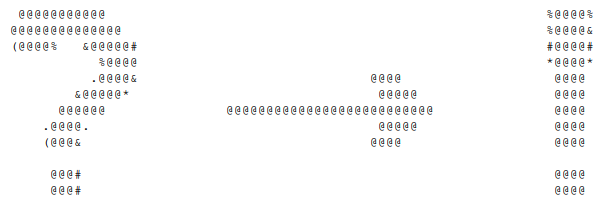
\includegraphics[width=\textwidth]{figures/kolloquium/kolloquium-ascii-art.png}
\end{minipage}
\end{figure}
\end{frame}

\end{document}